\documentclass[BA.tex]{subfiles}
\begin{document}
 This project \chk{concerns} the design and development of a teaching tool
 \chk{(from now on refered to as \tool)}
 to be used in the course `Logic in Computer Science' (\course) at the 
 University of Copenhagen. The tool is to be used in the teaching of
 natural deduction in \emph{propositional} logic, and allows users to
 write their proofs in English rather than the formal notation presented
 in the course textbook \book \cite{hr}.

Presenting students with a tool for writing natural deduction proofs
    in natural language is hoped to bridge the potential gap between
    understanding the structure and rules of natural deduction, and
    understanding the \emph{meaning} of the steps in such a process.
Furthermore, it is hoped that the
    presentation of such proofs in natural language will emphasize the
    \emph{independence} of the reached conclusion from the semantic 
    content of atomic declarative sentences: given \(p\) and \( p \ra q\),
    we may \emph{always} conclude \(q\)
    regardless of what declarative sentences $p$ and $q$
    represent. 
Finally, we believe that providing concrete and detailed 
    feedback through this \chk{validation tool} will not only
    help students learn from their mistakes, but also lower the risk of
    students getting stuck when working on their own, as well as lessen
    the work load of the TAs by catching many of the \chk{simpler}
    mistakes and thus allowing TAs to focus on students' understanding of
    the material rather than correcting \chk{typos}.

% Reader expectations
We expect readers to be familiar with \chk{\sml , as well as} the standard
 notation and terminology
 concerning the subjects \emph{parsing}, \emph{context-free grammars},
 and \emph{propositional logic} -- including Fitch-style notation
 for proofs. However, some of the specific
 tools used \chk{in} this project are briefly described below.

\subsubsection{Tools and programming language}
The \chk{development} part of the project is primarily written in the
 functional programming language \sml , using the \mos\
 \chk{implementation}. \chk{For readers unfamiliar with the module structure
 of \mos , functionality is implemented in \f{structures} stored in \f{.sml}
 files (a unit),
 and interfaces are implemented in \f{signatures} stored in \f{.sig}
 files\footnote{Or generated automatically, if no \f{.sig} file is
 provided.}.}
\paragraph{\yac} is ``a simple parser generator''\cite[p.~44]{mosman}
 that \chk{ships with} \mos .
 Given a context-free grammar specification with attached semantic actions,
 \yac\ produces a \f{.sml} file containing a \mos\ unit with code for
 a parser and a \f{.sig} file containing its interface
 \cite[\chk{\emph{ibid.}}]{mosman}.

\paragraph{\lex} is a lexer generator that \chk{ships with} \mos . It 
 \chk{takes} a set of regular expressions with attached semantic actions,
 and produces a \f{.sml} file containin \mos\ code for a lexical
 analyser\cite[p.~40]{mosman}. ``When used in conjunction with a parser
 generated by [\yac], the semantic actions compute a value belonging to
 the datatype \f{token} defined by the generated parsing 
 unit''\cite[\emph{ibid.}]{mosman}.

\paragraph{\bp \cite{box}} is the validation tool presently used in \course.
The \bp\ help-page\cite{boxhelp} gives the following
 description:
\begin{quote}
BoxProver is a userfriendly front-end to the Twelf\footnote{From
 the \s{Twelf} website\cite{twelf}: ``Twelf provides a uniform meta-language
 for specifying, implementing, and proving properties of programming
 languages and logics.''}proof assistant, and
 provides a simple way to encode and verify natural deduction proofs in
 propositional and first-order logic using Fitch-style notation. [...] 
 Besides verification, BoxProver also has facilities for producing visual
 representations of proofs, closely following the style and notation of
 the book \book, 2nd edition by Huth \& Ryan.
\end{quote}
Since this project \chk{deals with} \emph{propositional} logic, we do not
 concern ourselves with the \bp\ \chk{syntax} for first-order logic. 
 Thus, when we use the term `\bp\ syntax' in the following, it \chk{refers}
 to a subset that \chk{defines} natural deduction proofs in propositional
 logic, rather than the full syntax of \bp.

To illustrate the functionality of \bp , \fig{boxnfitch} shows an example
 of a Fitch-style proof (\subref{sf:fs}) and its encoding in \bp\ 
 (\subref{sf:boxin}) side by side; the visual representation provided by
 \bp\ is alsmost identical to the one shown in (\subref{sf:fs}).

\begin{figure}[!ht]
\centering
\begin{subfigure}[t]{0.45\textwidth}
\scriptsize
~\\
\(p \ra q \land r \vdash (p \ra q) \land (p \ra r)\)
\begin{logicproof}{2}
    p \ra q \land r & premise \label{1prm1}\\
        \begin{subproof}
        p & assumption \label{1p1}\\
        q \land r & \re{\ra} \ref{1p1}, \ref{1prm1}\\
        q & \re[1]{\land} \label{1q}
        \end{subproof}
    p \ra q & \ri{\ra} \ref{1p1}-\ref{1q} \label{1pgq}\\
        \begin{subproof}
        p & assumption \label{1p2}\\
        q \land r & \re{\ra} \ref{1p2}, \ref{1prm1}\\
        r & \re[2]{\land} \label{1r}
        \end{subproof}
    p \ra r & \ri{\ra} \ref{1p2}-\ref{1r} \label{1pgr}\\
    (p \ra q) \land (p \ra r) & \ri{\land} \ref{1pgq}, \ref{1pgr}
\end{logicproof}
~\\ %\vspace{-2mm}

\caption[]{Fitch-style}
\label{sf:fs}
\end{subfigure}
\(\qquad\)
\begin{subfigure}[t]{0.45\textwidth}
\scriptsize
\verbatiminput{imports/bpex121r}
\caption[]{\bp\ encoding}
\label{sf:boxin}
\end{subfigure}
\caption[Fitch-style proof and its \bp\ encoding]{An example of a
Fitch-style proof by natural deduction (\subref{sf:fs}) and its encoding
in \bp\ (\subref{sf:boxin})}
\label{boxnfitch}
\end{figure}

\subsubsection{Results}
The \chk{development} of this \tool\ \chk{consists} of three \chk{phases},
 handled \chk{separately}, but each building on the previous one. 

 The first of these is the definition of syntax\chk{, which is described in
 \afs{grams}}. To retain the \chk{rigor} of correct argumentation
 \chk{necessary} in formal proof construction, we define a \emph{subset}
 of the English language \chk{by} which users \chk{may express themselves} 
 rather than attempt to include the entire language. The subset does,
 however, read as natural language and thus the term
 `natural language' will be used to refer to this subset in the following,
 while `English'
 and `natural languages' (plural), will be used to respectively refer to
 the English natural language and natural languages in general. We also
 define and implement an abstract syntax for natural deduction proofs, as
 well as a formal syntax consistent with \bp\ notation.
 The \chk{relation} between the three syntax definitions is \chk{visualised}
 in \fig{syntaxes}.

\begin{figure}[!ht]
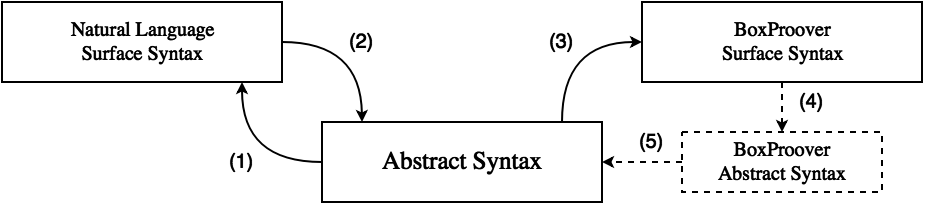
\includegraphics[width=\textwidth]{imports/SyntaxOverview}
\caption[Overview of \chk{project} syntax]{An overview of the syntax\chk{es}
defined in this project and the \chk{conversion} between them. The dashed
lines denote \bp\ tools and definitions not \chk{created} as part of
this project.
{\bf (1)} The \tool\ natural language pretty-printer renders an abstract
syntax proof in natural language with indentation.
{\bf (2)} The \tool\ parser takes natural language input and parses it
\chk{to} the abstract syntax.
{\bf (3)} The \tool\ formal \chk{pretty-printer} renders an abstract 
syntax proof in \bp\ surface syntax, with indentation for increased
readability.
{\bf (4)} \bp\ parses the surface syntax \chk{to its} internal abstract
syntax.
{\bf (5)} The \bp\ export tool \chk{converts} \bp\ abstract syntax to
\tool\ abstract syntax.
}
\label{syntaxes}
\end{figure}

\fig{syntaxes} also specifies the \chk{processes} that \chk{transform}
 proofs from one syntax to another. These parsing and
 unparsing functions denote the second phase, and 
 their \chk{design and implementation} is described in \afs{punp}.

 The final phase is the validation module, which provides the
 \chk{functionality} of the \tool. It is based on the abstract syntax,
 and the implementation of its key features is described in \afs{vmod}. 

 All three phases are combined in one program -- \f{Main} -- which provides
 the user interface, loads the appropriate modules and handles potential
 errors. The code for 
 \f{Main.sml} and the accompanyinng \f{Makefile} can be found in
 \app{Main} and \app[misc]{mkfile}, respectively. \FIX{Footnote instead?}
 The result is the multifunctional \tool . The current version provides
 three \chk{options for input}:
 \begin{description}
    \item[\f{print}] ~\\
 Pretty-prints a proof in natural language. This feature is currently
 implemented using a hardcoded dummy proof\footnote{Output 
 from the \bp\ export-tool pasted into the source code}
 titled ``boxproof'' as input to the printing function. 
    \item[\f{compare} <filename>] ~\\
 \chk{Preliminary implementation to test roundtrip functionality}. The
 current implementation parses the file specified by the \emph{filename}
 and compares the abstract syntax to that of the hardcoded dummy proof.
    \item[<filename>] ~\\
 validates natural deduction 
 proofs and produces a file containing either a \bp\ encoding of the proof,
 if it is valid, or a list of errors in the event that it is not.
 \end{description}
 
\subsubsection{Examples}
 Running \chk{\f{Main}} with the first option, \f{print}, produces the 
 pretty-printed natural language proof shown in \fig{nlprint}.

\begin{figure}[!ht]
~
\begin{subfigure}[t]{0.95\textwidth}
\footnotesize
\begin{tabbing}
boxproof:\\
We wish to prove (p\(\ra\)q)\(\lor\)(q\(\ra\)r).\\
In accordance with the law of the excluded middle, we introduce q\(\lor\)\(\neg\)q [1].\\
Ass\=ume \+ q [2].\\ 
	Ass\=ume \+ p [3].\\
		By copying 2, we get q here too [4].\\
	\< \- Discharge assumption [3].\\
	By applying the implication-introduction rule to [3]-[4], we get p\(\ra\)q [5].\\
	By applying the first or-introduction rule to [5], we get (p\(\ra\)q)\(\lor\)(q\(\ra\)r) [6].\\
\< \- Discharge assumption [2].\\
Ass\=ume \+ \(\neg\)q [7].\\
	Ass\=ume \+ q [8].\\
		By applying the negation-elimination rule to [8] and [7], we get \(\bot\) [9].\\
		By applying elimination of absurdity to [9], we get r [10].\\
	\< \- Discharge assumption [8].\\
	By applying the implication-introduction rule to [8]-[10], we get q\(\ra\)r [11].\\
	By applying the second or-introduction rule to [11], we get (p\(\ra\)q)\(\lor\)(q\(\ra\)r) [12].\\
\< \- Discharge assumption [7].\\
By applying the or-elimination rule to [1], [2]-[6], and [7]-[12], we get (p\(\ra\)q)\(\lor\)(q\(\ra\)r) [13].\\
\end{tabbing}

\end{subfigure}
\caption[]{An example of a natural deduction proof written in natural 
language}
\label{nlprint}
\end{figure}

 If the file containing that output is given as the second paramater when
 running \f{Main} with the second option, \f{compare} <filename>, the
 \tool\ returns the following:

 \coutput{imports/roundtrip.out}{compare.out}

 Which verifies that the unparser produces output that is accepted by the
 parser, and that the parser reproduces the original abstract syntax proof.
 The abstract syntax version of the proof is shown in \fig{bpexport}, and
 is the output produced by the \bp\ export tool.

 If, instead, the file with the natural language proof is given as the
 sole argument when running \f{main} with the third option, we get the
 following \chk{terminal} output from \tool :

 \coutput{imports/example.out}{example.out}
 The content of the output file is shown in \fig{bpinput}.

\begin{figure}[!ht]
\verbatiminput{imports/bpexport}
\caption[]{An example of an abstract syntax proof produced by the \bp\
export tool}
\label{bpexport}
\end{figure}

\begin{figure}[!ht]
~~
\begin{subfigure}[t]{0.95\textwidth}
\small
\verbatiminput{imports/bpimport}
\end{subfigure}
\caption[]{}
\label{bpinput}
\end{figure}

\subsubsection{Missing Component}
 As mentioned above, the current version of \tool\ uses a hardcoded
 dummy proof as the basis for the \f{print} and \f{compare} options.
 The functionality of the \bp\ export tool needs to be integrated in
 \tool\ in order to provide fully functional roundtripping.

\end{document}
